% ----------------------------  START --------------------------- 
\documentclass[../main]{subfiles} % main refers to main.tex
\graphicspath{{\subfix{../Illustrations}}}
\begin{document}
\addto\extrasfrench{\protected\edef:{\unexpanded\expandafter{:}}}
\selectlanguage{french}
% --------------------------------------------------------------- 
% Nombre de \contigs avec au moins n \SNP. L'ordonnée indique le nom de l'espèce considérée (\ref{model_bio}) et l'abscisse le \NbSNP considéré.  L'échelle de couleur indique le nombre de \contigs contenant ce \NbSNP.

\newgeometry{left=1cm, right=1cm, top=3cm, bottom=3cm}
\begin{landscape}
\begin{figure}[p]
    \centering
    \begin{subfigure}[b]{0.55\paperwidth}
        \centering
        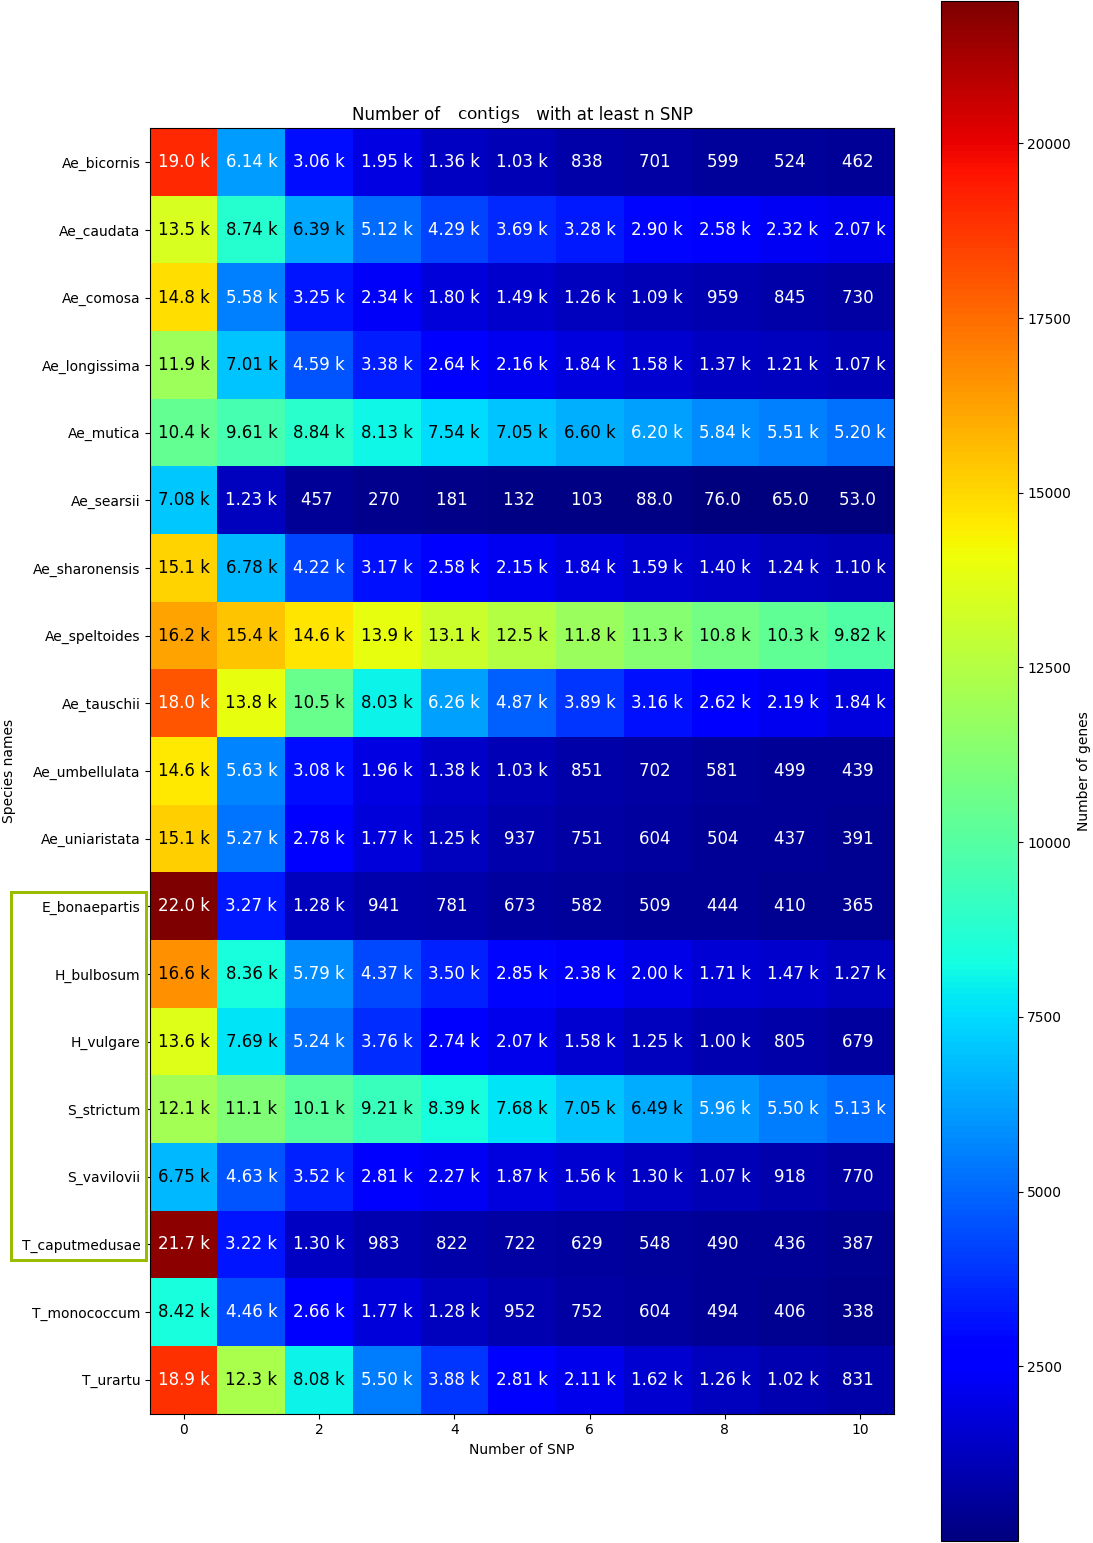
\includegraphics[width=\textwidth]{../Illustrations/Classic_Heatmap_SNP.png}
        \caption{Nombre de \contigs avec au moins $n$ \SNP. L'ordonnée indique le nom de l'espèce considérée (\ref{model_bio}) et l'abscisse le \NbSNP considéré. L'échelle de couleur indique le nombre de \contigs contenant ce \NbSNP. Les éspéces encadrées en jaune sont les éspéces appartenant à l'\gls{outgroup} (\cref{tab:Especes}). Image modifiée avec \gls{gimp}. \\
        Commande : \lstinline{Contig_name BiAllelic_SNP ./TargetedFiles.json -m 11 -kgqcuwt -j Classic --show_values -1 -y --transparent --legends legends.json --start_at_0}  
        }
        \label{fig:ClassicSNPHeatmap}
    \end{subfigure}
    \hfill
    \begin{subfigure}[b]{0.55\paperwidth}
        \centering
        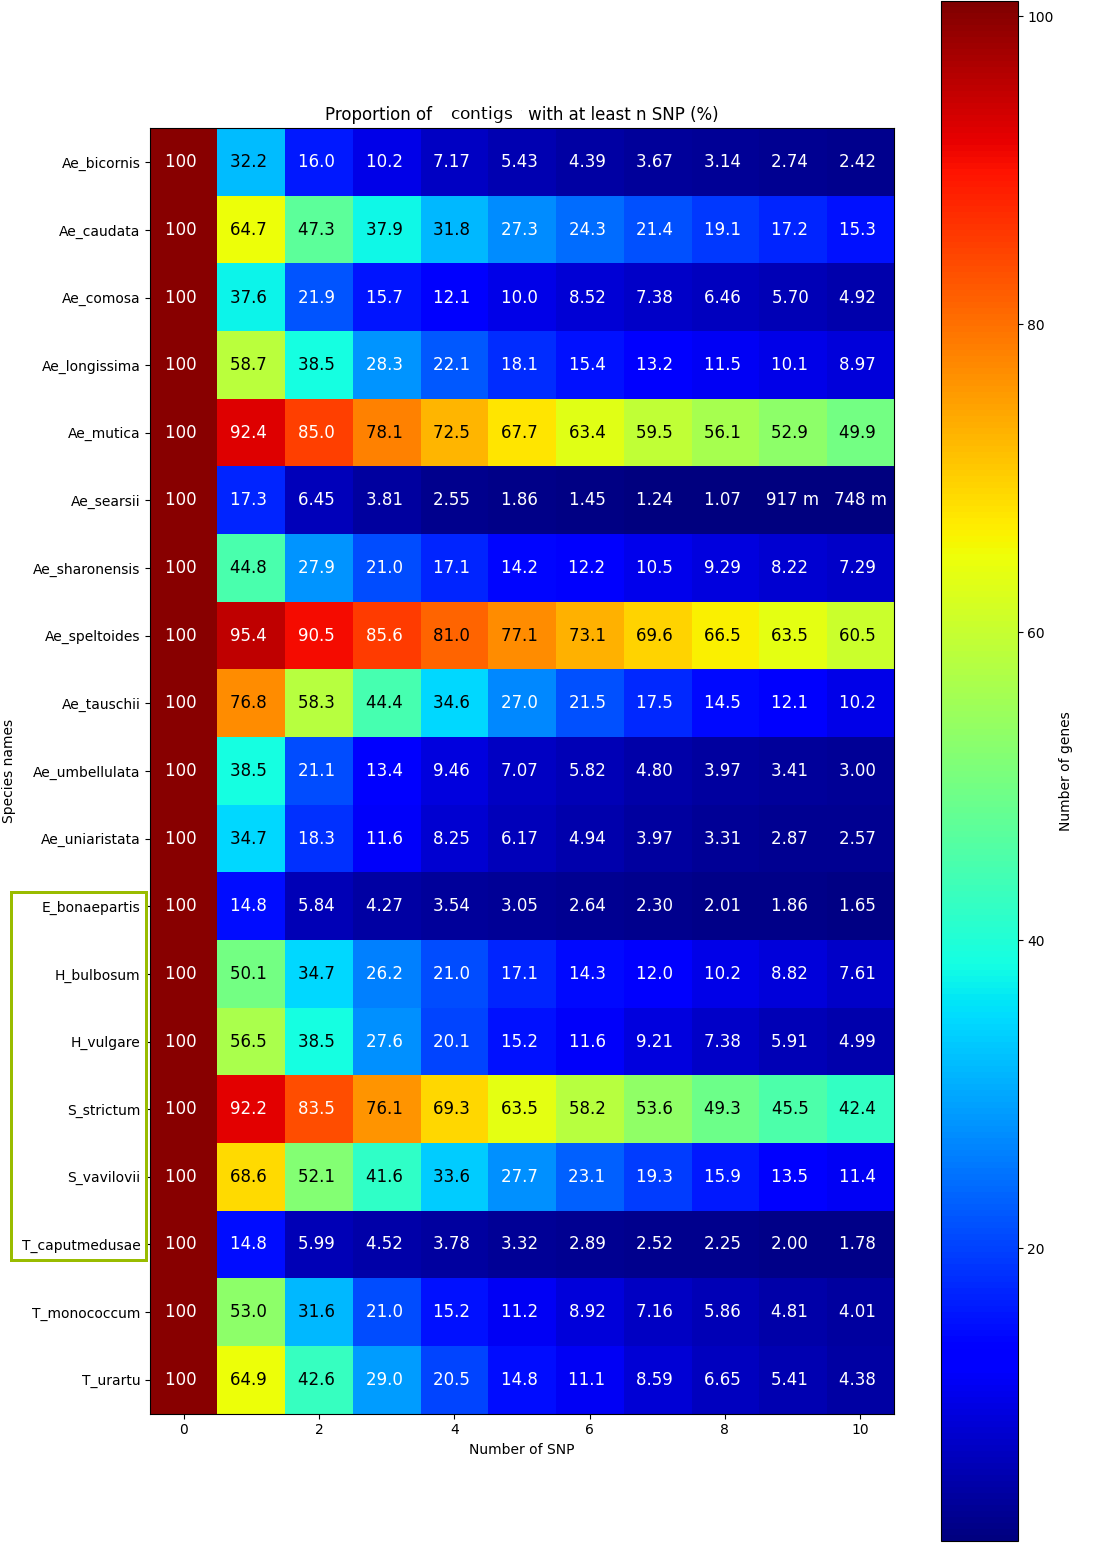
\includegraphics[width=\textwidth]{../Illustrations/Percent_Heatmap_SNP.png}
        \caption{Pourcentage de \contigs ayant au moins $n$ \SNP. L'ordonnée indique le nom de l'espèce considérée (\ref{model_bio}) et l'abscisse le \NbSNP considéré. L'échelle de couleur indique le pourcentage de \contigs contenant ce \NbSNP. Les éspéces encadrées en jaune sont les éspéces appartenant à l'\gls{outgroup} (\cref{tab:Especes}). Image modifiée avec \gls{gimp}.\\
        Commande : \lstinline{Contig_name BiAllelic_SNP ./TargetedFiles.json -m 11 -kgqcuwt -j Percent --show_values -1 -y --transparent --legends legends.json --start_at_0 --percent}
        }
        \label{fig:PercentSNPHeatmap}
    \end{subfigure}
    
    \caption{Résultat de l'analyse des \SNP (\ref{sec:SnpHeatmap}). Fait avec le logiciel mentionné dans la \ref{sec:SnpHeatmap}. La version utilisée est la 1.2.0.}
    \label{fig:SNPHeatmap}
    
\end{figure}
\end{landscape}
\restoregeometry
% --------------------------------------------------------------- 
\end{document}
% ----------------------------  END --------------------------- 
